\message{ !name(thesis.tex)}
% ----------------------------------------------------------------------
%                   LATEX TEMPLATE FOR PhD THESIS
% ----------------------------------------------------------------------

% based on Harish Bhanderi's PhD/MPhil template, then Uni Cambridge
% http://www-h.eng.cam.ac.uk/help/tpl/textprocessing/ThesisStyle/
% corrected and extended in 2007 by Jakob Suckale, then MPI-CBG PhD programme
% and made available through OpenWetWare.org - the free biology wiki


%: Style file for Latex
% Most style definitions are in the external file PhDthesisPSnPDF.
% In this template package, it can be found in ./Latex/Classes/
\documentclass[twoside,11pt]{Latex/Classes/PhDthesisPSnPDF}


%: Macro file for Latex
% Macros help you summarise frequently repeated Latex commands.
% Here, they are placed in an external file /Latex/Macros/MacroFile1.tex
% An macro that you may use frequently is the figuremacro (see introduction.tex)
% This file contains macros that can be called up from connected TeX files
% It helps to summarise repeated code, e.g. figure insertion (see below).

% insert a centered figure with caption and description
% parameters 1:filename, 2:title, 3:description and label
\newcommand{\figuremacro}[3]{
	\begin{figure}[htbp]
		\centering
		\includegraphics[width=1\textwidth]{#1}
		\caption[#2]{\textbf{#2} - #3}
		\label{#1}
	\end{figure}
}

% insert a centered figure with caption and description AND WIDTH
% parameters 1:filename, 2:title, 3:description and label, 4: textwidth
% textwidth 1 means as text, 0.5 means half the width of the text
\newcommand{\figuremacroW}[4]{
	\begin{figure}[htbp]
		\centering
		\includegraphics[width=#4\textwidth]{#1}
		\caption[#2]{\textbf{#2} - #3}
		\label{#1}
	\end{figure}
}

% inserts a figure with wrapped around text; only suitable for NARROW figs
% o is for outside on a double paged document; others: l, r, i(inside)
% text and figure will each be half of the document width
% note: long captions often crash with adjacent content; take care
% in general: above 2 macro produce more reliable layout
\newcommand{\figuremacroN}[3]{
	\begin{wrapfigure}{o}{0.5\textwidth}
		\centering
		\includegraphics[width=0.48\textwidth]{#1}
		\caption[#2]{{\small\textbf{#2} - #3}}
		\label{#1}
	\end{wrapfigure}
}

% predefined commands by Harish
\newcommand{\PdfPsText}[2]{
  \ifpdf
     #1
  \else
     #2
  \fi
}

\newcommand{\IncludeGraphicsH}[3]{
  \PdfPsText{\includegraphics[height=#2]{#1}}{\includegraphics[bb = #3, height=#2]{#1}}
}

\newcommand{\IncludeGraphicsW}[3]{
  \PdfPsText{\includegraphics[width=#2]{#1}}{\includegraphics[bb = #3, width=#2]{#1}}
}

\newcommand{\InsertFig}[3]{
  \begin{figure}[!htbp]
    \begin{center}
      \leavevmode
      #1
      \caption{#2}
      \label{#3}
    \end{center}
  \end{figure}
}


%%% Local Variables: 
%%% mode: latex
%%% TeX-master: "~/Documents/LaTeX/CUEDThesisPSnPDF/thesis"
%%% End: 




%: ----------------------------------------------------------------------
%:                  TITLE PAGE: name, degree,..
% ----------------------------------------------------------------------
% below is to generate the title page with crest and author name

%if output to PDF then put the following in PDF header
\ifpdf  
    \pdfinfo { /Title  (PhD and MPhil Thesis Classes)
               /Creator (TeX)
               /Producer (pdfTeX)
               /Author (YourName your@email.net)
               /CreationDate (D:YYYYMMDDhhmmss)  %format D:YYYYMMDDhhmmss
               /ModDate (D:YYYYMMDDhhmm)
               /Subject (xyz)
               /Keywords (add, your, keywords, here) }
    \pdfcatalog { /PageMode (/UseOutlines)
                  /OpenAction (fitbh)  }
\fi


\title{Title of your thesis}



% ----------------------------------------------------------------------
% The section below defines www links/email for author and institutions
% They will appear on the title page of the PDF and can be clicked
\ifpdf
  \author{\href{mailto:your@email.net}{YourName}}
%  \cityofbirth{born in XYZ} % uncomment this if your university requires this
%  % If city of birth is required, also uncomment 2 sections in PhDthesisPSnPDF
%  % Just search for the "city" and you'll find them.
  \collegeordept{\href{http://www.something.net}{CollegeOrDepartment}}
  \university{\href{http://www.something.net}{University}}

  % The crest is a graphics file of the logo of your research institution.
  % Place it in ./0_frontmatter/figures and specify the width
  \crest{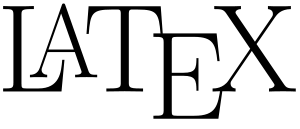
\includegraphics[width=4cm]{logo.png}}
  
% If you are not creating a PDF then use the following. The default is PDF.
\else
  \author{YourName}
%  \cityofbirth{born in XYZ}
  \collegeordept{CollegeOrDept}
  \university{University}
  \crest{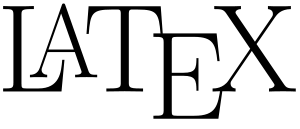
\includegraphics[width=4cm]{logo.png}}
\fi

%\renewcommand{\submittedtext}{change the default text here if needed}
\degree{Philosophi\ae Doctor (PhD), DPhil,..}
\degreedate{year month}


% ----------------------------------------------------------------------
       
% turn of those nasty overfull and underfull hboxes
\hbadness=10000
\hfuzz=50pt


%: --------------------------------------------------------------
%:                  FRONT MATTER: dedications, abstract,..
% --------------------------------------------------------------

\begin{document}

\message{ !name(thesis.tex) !offset(-3) }


%\language{english}

% sets line spacing
\renewcommand\baselinestretch{1.2}
\baselineskip=18pt plus1pt


%: ----------------------- generate cover page ------------------------

\maketitle  % command to print the title page with above variables


%: ----------------------- cover page back side ------------------------
% Your research institution may require reviewer names, etc.
% This cover back side is required by Dresden Med Fac; uncomment if needed.

\newpage
\vspace{10mm}
1. Reviewer: Name

\vspace{10mm}
2. Reviewer: 

\vspace{20mm}
Day of the defense:

\vspace{20mm}
\hspace{70mm}Signature from head of PhD committee:



%: ----------------------- abstract ------------------------

% Your institution may have specific regulations if you need an abstract and where it is to be placed in the document. The default here is just after title.


% Thesis Abstract -----------------------------------------------------


%\begin{abstractslong}    %uncommenting this line, gives a different abstract heading
\begin{abstracts}        %this creates the heading for the abstract page

Put your abstract or summary here, if your university requires it.

\end{abstracts}
%\end{abstractlongs}


% ---------------------------------------------------------------------- 


% The original template provides and abstractseparate environment, if your institution requires them to be separate. I think it's easier to print the abstract from the complete thesis by restricting printing to the relevant page.
% \begin{abstractseparate}
%   
% Thesis Abstract -----------------------------------------------------


%\begin{abstractslong}    %uncommenting this line, gives a different abstract heading
\begin{abstracts}        %this creates the heading for the abstract page

Put your abstract or summary here, if your university requires it.

\end{abstracts}
%\end{abstractlongs}


% ---------------------------------------------------------------------- 

% \end{abstractseparate}


%: ----------------------- tie in front matter ------------------------

\frontmatter
% Thesis Dedictation ---------------------------------------------------

\begin{dedication} %this creates the heading for the dedication page

To ...

\end{dedication}

% ----------------------------------------------------------------------
% Thesis Acknowledgements ------------------------------------------------


%\begin{acknowledgementslong} %uncommenting this line, gives a different acknowledgements heading
\begin{acknowledgements}      %this creates the heading for the acknowlegments

I would like to acknowledge the thousands of individuals who have coded for the LaTeX project for free. It is due to their efforts that we can generate professionally typeset PDFs now.

\end{acknowledgements}
%\end{acknowledgmentslong}

% ------------------------------------------------------------------------





%: ----------------------- contents ------------------------

\setcounter{secnumdepth}{3} % organisational level that receives a numbers
\setcounter{tocdepth}{3}    % print table of contents for level 3
\tableofcontents            % print the table of contents
% levels are: 0 - chapter, 1 - section, 2 - subsection, 3 - subsection


%: ----------------------- list of figures/tables ------------------------

\listoffigures	% print list of figures

\listoftables  % print list of tables


%: ----------------------- glossary ------------------------

% Tie in external source file for definitions: /0_frontmatter/glossary.tex
% Glossary entries can also be defined in the main text. See glossary.tex
% this file is called up by thesis.tex
% content in this file will be fed into the main document

% Glossary entries are defined with the command \nomenclature{1}{2}
% 1 = Entry name, e.g. abbreviation; 2 = Explanation
% You can place all explanations in this separate file or declare them in the middle of the text. Either way they will be collected in the glossary.

% required to print nomenclature name to page header
\markboth{\MakeUppercase{\nomname}}{\MakeUppercase{\nomname}}


% ----------------------- contents from here ------------------------

% chemicals
\nomenclature{DAPI}{4',6-diamidino-2-phenylindole; a fluorescent stain that binds strongly to DNA and serves to marks the nucleus in fluorescence microscopy} 
\nomenclature{DEPC}{diethyl-pyro-carbonate; used to remove RNA-degrading enzymes (RNAases) from water and laboratory utensils}
\nomenclature{DMSO}{dimethyl sulfoxide; organic solvent, readily passes through skin, cryoprotectant in cell culture}
\nomenclature{EDTA}{Ethylene-diamine-tetraacetic acid; a chelating (two-pronged) molecule used to sequester most divalent (or trivalent) metal ions, such as calcium (Ca$^{2+}$) and magnesium (Mg$^{2+}$), copper (Cu$^{2+}$), or iron (Fe$^{2+}$ / Fe$^{3+}$)}



 

\begin{multicols}{2} % \begin{multicols}{#columns}[header text][space]
\begin{footnotesize} % scriptsize(7) < footnotesize(8) < small (9) < normal (10)

\printnomenclature[1.5cm] % [] = distance between entry and description
\label{nom} % target name for links to glossary

\end{footnotesize}
\end{multicols}



%: --------------------------------------------------------------
%:                  MAIN DOCUMENT SECTION
% --------------------------------------------------------------

% the main text starts here with the introduction, 1st chapter,...
\mainmatter

\renewcommand{\chaptername}{} % uncomment to print only "1" not "Chapter 1"


%: ----------------------- subdocuments ------------------------

% Parts of the thesis are included below. Rename the files as required.
% But take care that the paths match. You can also change the order of appearance by moving the include commands.


\chapter{Introduction}
\label{cha:introduction}

\section{Background}
\label{sec:background}

The continuing evolution and commoditization of high-performance
computing infrastructure is constantly opening new horizons in spatial
modeling of human\slash environment interactions.  Increases in
processing throughput, affordability of tera- and petabyte-scale
storage resources, and ubiquity of parallelization tools and
techniques create opportunities for formulating models of spatial
processes of increasing extent, granularity, dimensionality, and
complexity.  The intersection of geography, economics, and computer
science is a fertile frontier where researchers capable of harnessing
the utility of available technology are presented with an
unprecedented opportunity to contribute to resolving the urgent
questions of our time regarding humankind's outlooks for survival,
stewardship, and prosperity in coming decades and centuries.  These
issues generally revolve around characterizations of our manipulation
of natural processes, notably food production; the side effects of
those activities, being alterations of biogeochemical fluxes of matter
and energy within and into the biosphere \citep{Sellers1997}; and the
economic exchanges that mediate these activities as modulated by
policy.  Meaningful abstractions of these processes in the form of
iterative, process-based models that we can formulate in order to
derive descriptions of their dynamics and forecasts of their unfolding
are not possible without some detailed, spatially explicit
characterization of the ecological disposition of the earth's surface.
This ecology is to be inclusive of human ecology, which is to say
settlement, development, utilization, and transformation of natural
resources.  The general form of such a characterization is a land
use\slash land cover (LULC) map which depicts landscapes according to
categories of anthropogenic and natural phenomena \citep{Fisher2005a}.
\todo{Warning--page numbers missing in Fisher2005a} These maps are
necessarily functions of history, climate, geology, hydrology and are
formulated according to some design or convention with regard to their
constituent types and their definitions, which make possible myriad
representations of a given landscape regardless of scale.  When
conducting analysis in this space it is typically necessary to tailor
the analysis to accommodate available data or create new data from raw
physical measurements and observations, but a third option of fusing
aspects of multiple available data sets is also available, as we will
demonstrate here.

Arguably the most significant intersection of land use and land cover
is agriculture.  Agricultural activity has transformed all but the
most inhospitable, impervious, and inaccessible corners of the globe
and serves as a crucial underpinning of civilization, but is still an
expression of variability in weather, soils, and biology, natural
phenomena beyond humans' control, across the face of the earth.  In
the face of uncertainty regarding food security, availability of raw
materials for industry and trade, impacts and dynamics of
deforestation, desertification, and climate change, and sensitivity to
these alarming trends due to a burgeoning global population, reliable
forecasts of agricultural production and productivity over the long
term are objects of much desire in the corridors of government,
finance, and industry.

Recent years have seen a significant increase in the availability of
global land cover data sets including the University of Maryland
Global Land Cover Classification, Global Land Cover 2000 (GLC2000),
and MODIS Land Cover Type (MLCT).  At the regional level the National
Land-cover Database (NLCD) provides high-resolution LULC data for the United States and Puerto Rico.  These data sets are
summarized in Table \ref{tab:lulc} with pertinent references and
attributes of their collection.  The proliferation of these data sets
reflects the diversification and technological advances among
space-borne sensors in recent years, resulting in improved resolution,
both spatial and temporal, as well as innovation in post-processing
and classification algorithms that transform raw sensor data into the
thematic data that is readliy applicable to theoretical modeling.

\begin{table}[ht]
  \begin{center}
    \begin{small}
%\begin{sidewaystable}
      \begin{tabular}{p{1in}p{1in}p{0.5in}lp{0.5in}}
        \hline
        Data set & Reference & Sensor & Resolution & Time Span \\
        \hline
        UMD GLobal Land Cover 1998 & \citet{Hansen2000} & AVHRR & 1km & 1981 -- 1994 (composite) \\
        Global Land Cover 2000 & \citet{EC2003,Bartholome2005} & SPOT & 1km & Nov~1999~--~Dec 2000 (composite) \\
        National Landcover Database (NLCD) & \citet{Homer2004,Homer2007} & Landsat & 30 m & 2001 \\
        MODIS Land Cover Type v005 & \citet{MLCT,Friedl2010} & MODIS (Aqua~\&~Terra) & 500m & 2001~--~2008 (annual~time~series) \\
        \hline
      \end{tabular}
    \end{small}
    \caption{Summary of global LULC data sets}
    \label{tab:lulc}
  \end{center}
\end{table}
%\end{sidewaystable}

\todo{Check format of \autoref{tab:lulc}}

Similarly there has also been a proliferation of data sets that
describe the distribution and intensity of global agricultural
activity.  Some such as the Global Irrigated Areas Map (GIAM)
\citep{Thenkabail2008} and the Global Map of Rainfed Crop Areas
(GMRCA) \citep{Biradar2009} are the product of applying classification
techniques to large collections of remote sensing and GIS data.
Others such as Agricultural Land in the Year 2000 (Agland200)
\citep{Ramankutty2008}, Harvested Area and Yields of 175 Crops
(175Crops2000) \citep{Monfreda2008}, and the Spatial Production
Allocation Model (SPAM) \citep{You2006} are further informed by
agricultural production data published at national and sub-national
levels and disaggregated to grid cells within those boundaries
according to an optimization method described by \citet{YouWood2006}.
Data sets such as these have the potential to complement those of the
general comprehensive LULC category by offering additional information
on how to differentiate areas of cropland according to cultivars, and
farming practices such as crop rotation, multiple cropping, and
irrigation.


\section{Objective}
\label{sec:objective}

The Community Integrated Model of Economic and Resource Trajectories
for Humankind (CIM-EARTH) project at the University of Chicago's
Computation Institute, \url{http://www.cimearth.org/}, seeks to
provide a framework in which to combine the best of modern
computational and economic science to guide climate and energy policy.
A major facet of this work involves forecasting of land use change
over coming decades in the face of market pressures and hypothetical
climate change scenarios.  The supply side of this market analysis
depends, among other industries, on agriculture.  Prices of
agricultural commodities are sure to change in years ahead in response
to changes in technology, both of production itself and the products
and materials that are derived from them, changes in aggregate demand
for food and its attendant political ramifications, and changes to the
environments where agricultural production occurs.  Rents and prices
of land will follow from the profitability, adaptiblity, and risks
associated with the commodities that are possible to produce on it, as
well as costs of energy and inputs needed to bring those goods to
market.  A spatially explicit model of not only agricultural
production, but also the conversion of land into and out of active,
profitable cultivation is needed in order to make statements about the
magnitude, trend, volatility, and sustainability of agricultural
output to guide decisions about investment and policy.  We call this
the Partial Equilibrium Economic Land-use (PEEL) model, which refers
to the assumption of long-term demand trajectories as given inputs and
calculates the likely distribution of production needed to meet that
demand.  The foundation of this modeling effort would have to be a
LULC data set that is ``complete'' in the sense that it assigns all
land plus coastal and inland water areas to one category or another,
and that differentiates among crops to provide a modeling environment
where shifts in production factor allocation can be driven by market
and physical variables.  None of the data sets considered so far
exhibit these qualities; the LULC data sets treat cropland as a
homogenous category and the agricultural maps do not depict other uses
and covers.  Hence the motivation to develop a hybrid data set that
satisfies these criteria.

The mathematical properties of the PEEL model dictate a somewhat
unconventional data model for representing the allocation of land area
to the various LULC\slash crop categories.  Rather than assigning
individual grid cells to discrete categories as is typically done for
LULC maps, PEEL is formulated in a sub-pixel analysis framework, such
that for each cell a fraction is assigned to each category to
represent the degree to which that LULC type is present across the
area of the grid cell.  In a tabular representation the data would
show cells in rows and the LULC types in columns with a constraint
that the values in each row sum to unity.  In terms of geospatial
mapping this is equivalent to assigning a layer or band in a stacked
image set to each category, as is done for spectral bands in
radiometric data, and applying the same sum-to-one constraint to each
pixel.  \sout{An advantage to this approach is that errors of false
  spatial precision in higher-resolution data sets from which our
  inputs are derived, meaning that pixels in the mother data set are
  aggregated into an expression of probability across the larger model
  grid cell versus the definite location implied by the thematic data.
  It also means that we will have an avenue for increasing model
  complexity and the raw size of the data set by a linear factor by
  increasing the depth of the data array rather than the quadratic
  increase that accompanies increases in resolution.} \todo{Does
  everyone agree that we can do without this passage?}  The primary
purpose of this design choice is to strike a balance between
locational specificity and a convenient accounting mechanism for land
use conversion forecasts that would only confer false precision and
impose additional computational burden if expressed spatially.  In
other words, the land area of a pixel is considered to be a single
location whose internal arrangement is unspecified.  The model can
incorporate constraints governing the iterative transition of those
fractions that are stated algebraically in order to exclude protected
natural areas from conversion or require a degree of autocorrelation
among neighbors to prevent unrealistic divergences in development
patterns among grid cell neighborhoods, for example.

A disadvantage of this data model is apparent when attempting to
visualize the data.  A thematic map can be viewed in a single pass
given a well-designed palette that has a reasonable number of classes
and the relative proportions and distributions of classes can be
readily perceived by the viewer.  For the sub-pixel data model a
cognitive adjustment is necessary in order to consider multiple
classes simultaneously.  Although it is possible to employ the
false-color approach typically used for viewing multispectral data,
which is to map a subset of three bands to the red, green, and blue
channels, this limits a given map to portraying three classes
simultaneously, or else picking two of primary interest and lumping
the remaining fractions into a catch-all category.  This method is not
quite as applicable to categorical data that we are discussing as it
is to spectral data because a set of three spectral bands are
typically left in long-to-short wavelength order and reassigned to
red, green, and blue, which amounts to shifting their frequencies into
the visible spectrum, in order to produce a false-color image.  It
would be difficult to interpret the mixing of thematic hues or the
arbitrary assignment of categories to primary hues.  The approach to
visualization taken for this paper is to render maps in individual
layers with a uniform palette to express the fractional expression of
the classes and distinguish zero from null outside the set of pixels
included by the analysis mask.  Interpretation is aided by presenting
these maps in collections called facets in Wilkinson's
\citeyearpar{Wilkinson2005} grammar of graphics to convey the full
depth of information in consideration.

Given that the CIM-EARTH modeling framework is in a prototype phase we
are taking a conservative posture towards the degree of detail that we
wish to capture in early applications.  This is expressed by the
choice of resolution of our model grid and the number of LULC
categories, including crop sub-categories, to which each cell can be
allocated.  With an ultimate goal of running simulations at global
extents we wanted to err on the side of prudence before measuring the
computational requirements of processing time and storage of a working
prototype.  Early tests gauging the computational requirements for
carrying out these simulations have indicated that operating on a 5$'$
grid cell globally is not prohibitively costly in time, memory, or
storage and that the design, implement, evaluate iterative development
cycle can proceed at a satisfactory pace.  This choice of resolution
is not as arbitrary as it may seem given that it equates to roughly
10km at the equator and happens to be the same resolution as some of
the base data employed in this exercise.

The algorithm described here will be peformed on the subset of the
global 5-arc-minute grid that contain land area of the 48 contiguous
states of the United States but is intended to be applied globally.
As we will discuss in Chapter \ref{cha:datasets} when the base data
sets are described in greater detail the MLCT is chosen as the
foundation of this method because of its global coverage and greatest
resolution among global data products.  As the technique presented in
Chapter \ref{cha:analysis} matures it will be applied globally and
also extended in time to convert the proceeding years of the MLCT time
series to a form useful in the PEEL model.  This will be important for
model validation to show that the model is capable of producing an
evolution of the overall state of land use that corresponds to
available observations.  As we will see the necessary information
needed to obtain a realistic distribution of areas for all classes is
not currently available.  We use the NLCD to complement MLCT for
certain classes that are too small to resolve at 500m, hence the
restricted extent for which this method is currently feasible.  In
Chapter \ref{cha:conclusions} we wrap up with a discussion of the
merits of this endeavor and propose future avenues of research based
thereon.

At this time we are not aware of any other systematic attempt to
incorporate the full depth of information offered by MLCT, which is a
collection of three map layers: a primary cover class, a confidence
level for that primary classification, and a secondary classification.
Rather than interpret the secondary classification as the next most
likely possibility we accept this triplet as an expression of the
sub-pixel composition of that area.  Aggregation of MLCT from 15
$''$ to 5$''$ will blur the spatial precision implied
by this formula and treat the local $20 \times 20 \times 3$ array as a
probabilistic expression of the local landscape composition.  We will
show that this approach, given a principled assumption about the
relationship between confidence level and sub-pixel area, that
aggregate acreage estimates of the LULC classes, particularly
cropland, are improved through this method.  More on this in Section~\ref{sec:mlct}.

\section{Reproducible Research}
\label{sec:reproducible}

We maintain that the manner in which we execute this analysis is as
significant, if not more so, to the practice of geospatial analysis as
the product of the analysis itself.  The second objective of this
paper is to demonstrate the concept of reproducible resarch in
geospatial analysis that has been made possible by a suite of
open-source software tools.  Previous to employing the suite of tools
described below, our typical research experience with widely available
GIS software, both free and commerical, is to conduct the analysis in
a graphical user interface (GUI) environment and capture outputs for
publication by manually exporting maps and charts as images and
transcribing quantitative results from on-screen displays into the
body of a document.  Whenever an adjustment is made the maps, charts,
tables, and quantities in the paper must be updated manually.  The
open-source GIS software package
\href{http://grass.osgeo.org/}{\texttt{GRASS}} \citep{GRASS} employs a
command-line oriented interface as its basic mode of user interaction
which makes recording of steps in an analysis in the form of a script
a more approachable undertaking once the user develops familiarity
with the necessary commands, but due to \texttt{GRASS}'s decades-long Unix
heritage, this scripting is done using the Bash shell, a system that
was designed primarily for system administration and suffers from a
byzantine syntax and a dearth of native data structures, making
succinct, expressive programming difficult.

The \href{http://www.r-project.org/}{\texttt{R}} statistical package
addresses these shortcomings \citep{R} by virtue of its design's
orientation towards mathematical and statistical analysis.  Using
Robert Hijmans' \citeyearpar{Hijmans2011} \texttt{raster} package for
\texttt{R} provides an interface for accessing and analyzing
geospatial raster data sets without being forced to load the entire
data set into memory, a constraint that has historically been the case
with \texttt{R} data in general and made operations on large
geospatial data sets difficult.  Friedrich Leisch's
\citeyearpar{Leisch2002} \texttt{Sweave} package for \texttt{R} is a
tool for embedding \texttt{R} code within a
\href{http://www.latex-project.org/}{\LaTeX} \citep{Lamport1994}
document for inline code evaluation and dynamic injection of figures,
tables, and text into a document prior to final typesetting.  The
utilization of these tools results in a software environment where the
princples of reproducible research described and demonstrated by
\citet{Gentleman2007} can be applied.  An academic paper produced
under this paradigm is analogous to a piece of open-source software
where the majority of ``users'' will simply want the ``compiled''
version in the form of a PDF document, but the author also provides
access to the the source code behind the production of that document
for inspection, re-execution, and adaptation for follow-on research.
This approach lowers the costs of reproduction and verification of
scientific analyses, central tenets of the scientific method that have
effectively fallen out of practice due to these costs.  With the
advent of software tools such as these this approach to documenting
research has gained a foothold in numerous desciplines from statistics
to medical imaging.

The tables, charts, and maps included in this document are generated
by \texttt{R} code which will be included as an appendix.  The maps
and charts are produced using Hadley Wickham's
\citeyearpar{Wickham2009} \texttt{ggplot2} package, employing the
grammar of graphics mentioned above.  David Dahl's \texttt{xtables}
package is used to convert \texttt{R} data frames into tables
marked-up for typesetting.  \texttt{Sweave} itself provides a facility
for injecting the results of evaluating arbitrary \texttt{R}
expressions in the text body, making it possible to render pieces of
data, such as total acreages, in a dynamic fashion within the body of the text.

The source code of this paper will be submitted on optical media to
Northeastern Illinois University's Graduate college along with the
final draft.  It will also be available via GitHub at
\url{https://github.com/nbest937/thesis}.  The initial, intermediate,
and final data products will be made available for download either
through \url{http://www.ci.uchicago.edu/~nbest} and\slash or
\url{http://www.cimearth.org/} by request to
\url{mailto:nbest@ci.uchicago.edu} or \url{mailto:nbest@alum.mit.edu}.
	% background information
% this file is called up by thesis.tex
% content in this file will be fed into the main document

\chapter{Aims of the project} % top level followed by section, subsection


% ----------------------- contents from here ------------------------

\section{Final aim}

Our ultimate goal is...

\section{Preliminary aims}

There will be several preliminary scientific targets to be accomplished on the way...




% ---------------------------------------------------------------------------
% ----------------------- end of thesis sub-document ------------------------
% ---------------------------------------------------------------------------						% aims of the project

\include{3/XYZ}			
\include{4/XYZ}	
\include{5/XYZ}
\include{6/XYZ}

% this file is called up by thesis.tex
% content in this file will be fed into the main document

\chapter{Discussion} % top level followed by section, subsection


% ----------------------- paths to graphics ------------------------

% change according to folder and file names
\ifpdf
    \graphicspath{{7/figures/PNG/}{7/figures/PDF/}{7/figures/}}
\else
    \graphicspath{{7/figures/EPS/}{7/figures/}}
\fi


% ----------------------- contents from here ------------------------






% ---------------------------------------------------------------------------
% ----------------------- end of thesis sub-document ------------------------
% ---------------------------------------------------------------------------               % discussion of results


% this file is called up by thesis.tex
% content in this file will be fed into the main document

\chapter{Materials \& methods} % top level followed by section, subsection


% ----------------------- paths to graphics ------------------------

% change according to folder and file names
\ifpdf
    \graphicspath{{8/figures/PNG/}{8/figures/PDF/}{8/figures/}}
\else
    \graphicspath{{8/figures/EPS/}{8/figures/}}
\fi

% ----------------------- contents from here ------------------------




 

% ---------------------------------------------------------------------------
%: ----------------------- end of thesis sub-document ------------------------
% ---------------------------------------------------------------------------



 






        % description of lab methods




% --------------------------------------------------------------
%:                  BACK MATTER: appendices, refs,..
% --------------------------------------------------------------

% the back matter: appendix and references close the thesis


%: ----------------------- bibliography ------------------------

% The section below defines how references are listed and formatted
% The default below is 2 columns, small font, complete author names.
% Entries are also linked back to the page number in the text and to external URL if provided in the BibTex file.

% PhDbiblio-url2 = names small caps, title bold & hyperlinked, link to page 
\begin{multicols}{2} % \begin{multicols}{ # columns}[ header text][ space]
\begin{tiny} % tiny(5) < scriptsize(7) < footnotesize(8) < small (9)

\bibliographystyle{Latex/Classes/PhDbiblio-url2} % Title is link if provided
\renewcommand{\bibname}{References} % changes the header; default: Bibliography

\bibliography{9_backmatter/references} % adjust this to fit your BibTex file

\end{tiny}
\end{multicols}

% --------------------------------------------------------------
% Various bibliography styles exit. Replace above style as desired.

% in-text refs: (1) (1; 2)
% ref list: alphabetical; author(s) in small caps; initials last name; page(s)
%\bibliographystyle{Latex/Classes/PhDbiblio-case} % title forced lower case
%\bibliographystyle{Latex/Classes/PhDbiblio-bold} % title as in bibtex but bold
%\bibliographystyle{Latex/Classes/PhDbiblio-url} % bold + www link if provided

%\bibliographystyle{Latex/Classes/jmb} % calls style file jmb.bst
% in-text refs: author (year) without brackets
% ref list: alphabetical; author(s) in normal font; last name, initials; page(s)

%\bibliographystyle{plainnat} % calls style file plainnat.bst
% in-text refs: author (year) without brackets
% (this works with package natbib)


% --------------------------------------------------------------

% according to Dresden med fac summary has to be at the end
%
% Thesis Abstract -----------------------------------------------------


%\begin{abstractslong}    %uncommenting this line, gives a different abstract heading
\begin{abstracts}        %this creates the heading for the abstract page

Put your abstract or summary here, if your university requires it.

\end{abstracts}
%\end{abstractlongs}


% ---------------------------------------------------------------------- 


%: Declaration of originality

% Thesis statement of originality -------------------------------------

% Depending on the regulations of your faculty you may need a declaration like the one below. This specific one is from the medical faculty of the university of Dresden.

\begin{declaration}        %this creates the heading for the declaration page

I herewith declare that I have produced this paper without the prohibited assistance of third parties and without making use of aids other than those specified; notions taken over directly or indirectly from other sources have been identified as such. This paper has not previously been presented in identical or similar form to any other German or foreign examination board.

The thesis work was conducted from XXX to YYY under the supervision of PI at ZZZ.

\vspace{10mm}

CITY,


\end{declaration}


% ----------------------------------------------------------------------



\end{document}

\message{ !name(thesis.tex) !offset(-262) }
